\documentclass[conference]{IEEEtran}
\IEEEoverridecommandlockouts
% The preceding line is only needed to identify funding in the first footnote. If that is unneeded, please comment it out.
\usepackage{cite}
\usepackage{amsmath,amssymb,amsfonts}
\usepackage{algorithmic}
\usepackage{graphicx}
\usepackage{textcomp}
\usepackage{xcolor}
\usepackage{booktabs}
\usepackage{subcaption}
\usepackage{lipsum} 
\usepackage{dblfloatfix}
\def\BibTeX{{\rm B\kern-.05em{\sc i\kern-.025em b}\kern-.08em
    T\kern-.1667em\lower.7ex\hbox{E}\kern-.125emX}}

\begin{document}

% Title
\title{Development of Microcontroller-Based AI Robot Tour Guide Utilizing Custom Language Models}

% funding footnote -- need?
% {\footnotesize \textsuperscript{*}Note: Sub-titles are not captured in Xplore and
% should not be used}
% \thanks{Identify applicable funding agency here. If none, delete this.}
% }

% Authors 
\author{
    \IEEEauthorblockN{Ian S. Jackson}
    \IEEEauthorblockA{\textit{Lane Department of Computer Science and Electrical Engineering} \\
    \textit{West Virginia University}\\
            Morgantown, United States \\
            isj0001@mix.wvu.edu}
    % \and
    % \IEEEauthorblockN{2\textsuperscript{nd} Given Name Surname}
    % \IEEEauthorblockA{\textit{dept. name of organization (of Aff.)} \\
    % \textit{name of organization (of Aff.)}\\
    %         City, Country \\
    %         email address or ORCID}
    % \and
    % \IEEEauthorblockN{3\textsuperscript{rd} Given Name Surname}
    % \IEEEauthorblockA{\textit{dept. name of organization (of Aff.)} \\
    % \textit{name of organization (of Aff.)}\\
    %         City, Country \\
    %         email address or ORCID}
    % \and
}

\maketitle
\thispagestyle{plain}
\pagestyle{plain}

%== ABSTRACT ==%
\begin{abstract}
    This paper presents the development of a microcontroller-based AI robotic tour guide designed to enhance visitor engagement at educational institutions. 
    Leveraging custom small language models (SLMs), the system delivers real-time, conversational interactions tailored to prospective students. 
    The model, fine-tuned on a curated dataset of questions and answers related to department offerings, integrates with a robotic platform equipped with microphone and speaker interfaces. 
    Evaluation of two candidate models, FLAN-T5 and BART, highlights trade-offs between accuracy, conversational quality, and response time. 
    The implementation demonstrates the feasibility of deploying compact and efficient AI solutions on edge devices, providing a scalable and interactive tool for showcasing departmental advancements. 
    Future work aims to refine deployment on resource-constrained hardware and refining models for better results.
\end{abstract}

%== KEYWORDS ==%
% \begin{IEEEkeywords}
%     TODO: keywords
% \end{IEEEkeywords}

%== Introduction ==%
\section{Introduction}
Advancements in artificial intelligence (AI) and robotics have revolutionized the way interactive experiences are crafted across various domains. 
Educational institutions, in particular, stand to benefit from these technologies by enhancing engagement with prospective students. 
The integration of AI-powered robots as tour guides presents a novel approach to showcase departmental offerings in an interactive and personalized manner.

The Computer Science and Electrical Engineering (CSEE) department seeks to transform the traditional tour experience into an immersive journey through its cutting-edge research and innovations. 
By deploying an AI-powered robotic tour guide, prospective students are offered a unique opportunity to interact with the very technologies that define the department's forefront position in the field. 
This interactive platform not only conveys information about programs and facilities but also provides a tangible demonstration of the department's advancements, allowing visitors to experience firsthand the innovative spirit and technological prowess that drive the CSEE department.

This research project focuses on the development of a custom language model hosted on a microcontroller, drawing on the principles of small language models (SLMs). 
The language model is trained on a curated dataset of questions and answers pertinent to the CSEE department's programs, faculty, research areas, and facilities. 
By implementing the model on a microcontroller, we achieve a compact and efficient system suitable for real-time conversational exchanges within a robotic platform.

The robot is equipped with a simple microphone and speaker interface, facilitating natural language communication with users. 
Prospective students can engage in verbal interactions, asking questions and receiving informative responses from the robot. 
This paper outlines the design and implementation of the custom language model, the integration with robotic hardware, and an evaluation of the system's effectiveness in enhancing visitor engagement and providing valuable information.

%== Related Work ==%
\section{Related Work}
The integration of small language models (SLMs) into robotic platforms for enhanced human-robot interaction, particularly in educational settings, presents unique challenges and opportunities.
While large-scale foundation models (FMs) like Llama \cite{b1} and Mixtral \cite{b2} have revolutionized natural language processing, their size and computational requirements make them unsuitable for resource-constrained edge devices. 
The emergence of SLMs aims to address this gap, offering compact models with tens to hundreds of millions of parameters \cite{b3}, suitable for development on microcontrollers. 

\begin{figure*}[t]
    \centering
    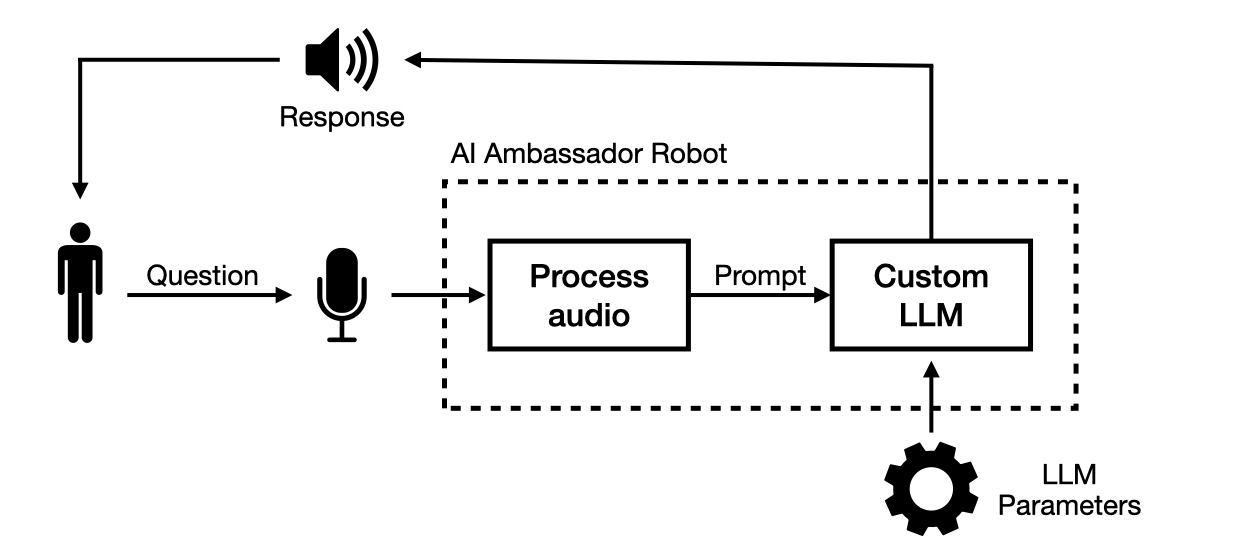
\includegraphics[width=0.8\linewidth]{assets/diagram.001.jpeg}
    \caption{AI Robot System Diagram}
    \label{fig:system}
\end{figure*}

%== Our approach ==% 
\section{Our Approach}
\subsection{Hardware}
Various mediums to house the underlying AI-powered tour guide. The mediums can be broken up into two categories: kit based systems and custom systems.
The first kit-based system is the MangDang Mini Pupper \cite{b4}, an open-source dog-like robot, powered by a Raspberry Pi. It highlights a simple and quick assembly as well as an all-inclusive kit. 
The second kit-based system is the Poppy Humaniod \cite{b5}, and open-source human-like robot. The Poppy Humaniod is powered by a Raspberry Pi as well, however most of the parts are 3D printed by the customer. The robot utilizes Dynamixel servos to provide stable and accurate movement, the downside being the high cost of the parts.
The last medium considered is a custom system, designed from scratch. This opens up the possibility for the robotic medium to be custom to the department and college. 

Regardless of the robotic medium chosen, the robot will feature three main parts to facilitate an interactive experience: a microphone, a computer, and a speaker. 
A simplified system diagram can be seen in Figure \ref{fig:system}. The prospective student will interact with the LLM via the microphone, where their question will be translated from audio to text.
This question is then fed into the LLM as a prompt. Once the LLM processes the prompt and outputted back to the prospective student via a speaker.

\subsection{Custom Language Models}
The core of the AI-powered robotic tour guide is a custom language model designed to facilitate natural and informative conversations with prospective students. 
To meet the project's objectives, the language model was developed with the following criteria in mind: it had to be open source, capable of effective training on both question-and-answer (Q\&A) datasets and web page content, and optimized for lightweight deployment with quick response times on a microcontroller platform.

\noindent
\textbf{Selection of the Language Model:} 
An open-source language model was chosen due to their capabilities in lightweight implementations while maintaining high-quality natural language understanding and generation.
Open-source models such as FLAN-T5 \cite{b6} and BART \cite{b7} provide a solid foundation due to their small size and performance on Q\&A task with minimal fine-tuning. 
These models are well-suited for customization and can be fine-tuned with domain-specific data.

Fine-tuned Langauge Agnostic Network (FLAN-T5) is a variant of the T5 (Text-to-Text Transfer Transformer) model, which is pretrained on a diverse range of tasks. 
It features strong ability to be trained on a wide variety of datasets, including Q\&A tasks. 
It also meets the versatile, scalability, and open-source criteria.

Bidirectional and Auto-regressive Transformer (BART) is a sequence-to-sequence model optimized for tasks like text generation, summarization, and translation. 
It combines bidirectional context encoding with autoregressive decoding. 
It features capabilities to fine-tune on specific datasets, and effective in both understanding and generating coherent responses.
Like FLAN-T5, it meets the criteria concerned with being open-source, scalable, and versatile.

\noindent
\textbf{Training on Q\&A and Web Page Datasets:} The model was trained on a curated Q\&A dataset comprising frequently asked questions by prospective students and their corresponding answers. 
This dataset was created with content scraped from the department's web pages, including program descriptions, faculty profiles, research highlights, and facility overviews. 
Each Q\&A pair that was human generated, was fed into ChatGPT to augment and expand on the dataset. ChatGPT would take in a single Q\&A pair and create multiple copies but using differing language to expand and diversify the dataset.
ChatGPT would then output the augmented data in the Stanford Question Answering Dataset (SQuAD) format \cite{b8}.

The SQuAD format includes a list of topics as the top level, with each topic having a title. In each topic exist paragraphs, these contain context to the topic and question-answer pairs.
To fit the dataset to the task at hand, the topics were chosen based off of types of questions that could be asked about the department:
degree programs, research opportunities, facilities and resources, clubs and organizations, career opportunities, internships, financial aid and scholarships, faculty information, admission process, and location and contact.
Under each of these topics, question-answer pairs are generated and augmented to expand the dataset. 
The resulting dataset included 263 question-answer pairs.

%== Methodology ==%
\section{Methodology}
Both FLAN-T5 and BART were finetuned on the same custom dataset. The model hyperparameters can be found in Table \ref{tab:hyperparams}.
The test dataset included eight questions pertaining to the CSEE department, topics of the questions including: degree programs, research opportunities, student organizations, and career opportunities. 


\begin{table}[!ht]
    \centering
    \caption{Hyperparameters for FLAN-T5 and BART Fine-Tuning}
    \label{tab:hyperparams}
    \begin{tabular}{l|c|c}
        \toprule
        \textbf{Hyperparameter}         & \textbf{FLAN-T5}         & \textbf{BART} \\
        \midrule
        Evaluation Strategy             & Epoch                   & Epoch                     \\ 
        Weight Decay                    & 0.01                    & 0.01                      \\ 
        Learning Rate                   & 5e-5                    & 3e-5                      \\ 
        Logging Steps                   & 5                       & 5                         \\ 
        Train Batch Size                & 8                       & 8                         \\ 
        Evaluation Batch Size           & 8                       & 8                         \\ 
        Number of Training Epochs       & 10                      & 5                         \\ 
        \bottomrule
    \end{tabular}
\end{table}

\subsection{Language Model Evaluation and Selection}
To evaluate the performance of FLAN-T5 and BART, two metrics are employed: F1 Score and BLEU score. 
These metrics provide insight to the models' precision, recall, and accuracy in text understanding and generation tasks.
Another metric used to evaluate the model is average response time, or the mean of the time it takes to process an input and provide an output over all test data.

\noindent
\textbf{F1 Score:}
The F1 Score is a harmonic mean of precision and recall, offering a single metric to evaluate a model's ability to balance false positives and false negatives.
The calculation for the F1 Score is seen in Equation \ref{eq:F1}.

\begin{equation} \label{eq:F1}
    \text{F1} = 2 \cdot \frac{P \cdot R}{P + R}
\end{equation}

\noindent
where $P$ is the precision and $R$ is the recall over the test dataset. 

\noindent
\textbf{BLEU Score:}
The Bilingual Evaluation Understudy (BLEU) Score measures the quality of the text generated by comparing it with one or more of the reference texts.
It assesses how similar the generated text is to human-provided references, in this case the reference is the provided answer to the test question. 
The BLEU Score formula is seen in Equation \ref{eq:BLEU}.

\begin{equation} \label{eq:BLEU}
    \text{BLEU} = \text{BP} \cdot \exp \left( \sum_{n=1}^{N} w_n \log(p_n) \right)
\end{equation}
\begin{equation} \label{eq:BP}
    \text{BP} = 
    \begin{cases}
        1, & c > r \\
        e^{1 - r/c}, & c \leq r
    \end{cases}
\end{equation}
\noindent
where $\text{BP}$ is the Brevity Penalty (seen in Equation \ref{eq:BP}), $p_n$ is the precision of $n$-grams, and $w_n$ is the weight associated to $n$-grams (typically equal $\forall n$).

\subsection{Deployment}
The implementation of FLAN-T5 and BART leverages Hugging Face Transformers, a comprehensive framework for working with pre-trained language models.
Training was done via the Hugging Face training pipeline, built on the Trainer class and text generation was configured for inference using the Hugging Face pipeline for text generation.
Each model utilized their own transformer: The T5 Tokenizer \cite{b9} for FLAN-T5 and BART Tokenizer \cite{b10} for BART.

For development purposes, all training and evaluation was done on a 2020 Macbook Pro with a Quad-Core Intel i7 processor. 
There are obvious limitations to the machine, especially in terms of training and developing a LLM. 
Once the model's are finalized in terms of training and evaluation, the custom LLM will be moved to an edge device for further evaluation. More discussed in Future Work.

%== Results ==%
\section{Results}
Both FLAN-T5 and BART were trained on the custom dataset with the hyperparameters seen in Table \ref{tab:hyperparams}. 
A sample of the output from FLAN-T5 and BART can be seen in Figure \ref{fig:FLAN_Out} and Figure \ref{fig:BART_Out}, respectively.
While FLAN-T5 performs fairly well on questions about degree programs offered, research opportunities, and student organizations, it lacks in responses pertaining to careers.
BART does well with student organization questions, but lacks elsewhere. Notably, mentioning University of California, Davis when asked about research. 

Figure \ref{fig:eval_loss} compares the evaluation performance of the two models over the epochs trained.
BART achieves lower overall evaluation loss by the end of the training, indicating better generalization to the evaluation dataset compared to FLAN-T5.
Figure \ref{fig:train_loss} highlights the training dynamics of the two models. 
FLAN-T5 stabilizes at a slightly higher training loss compared to BART by the end of training. However, its loss curve demonstrates greater consistency, possibly reflecting better robustness against overfitting.

\begin{figure}[h]
    \centering
    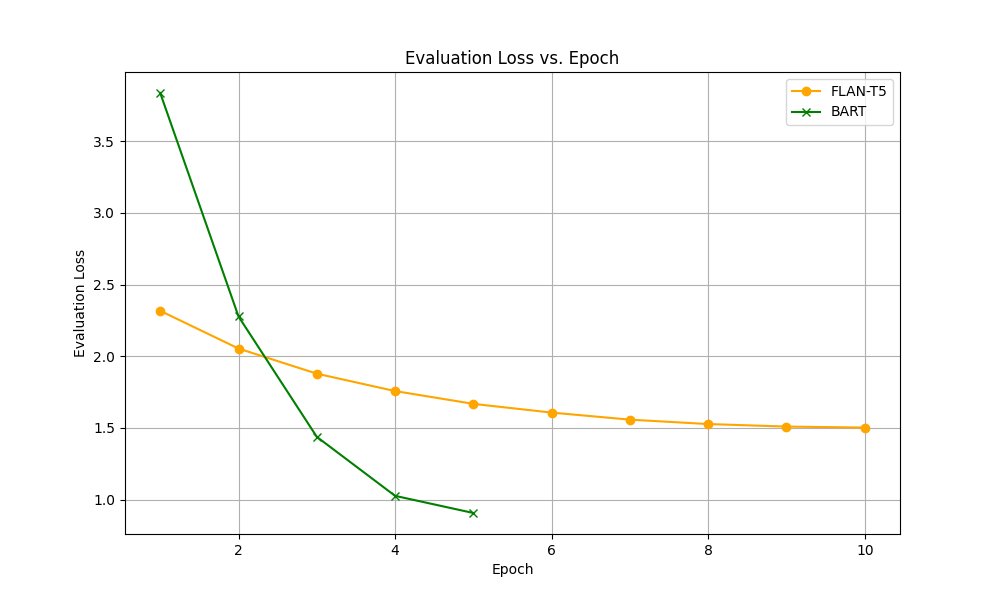
\includegraphics[width=\linewidth]{assets/eval_loss.png}
    \caption{Evaluation Loss vs Epoch}
    \label{fig:eval_loss}
\end{figure}

\begin{figure}[h]
    \centering
    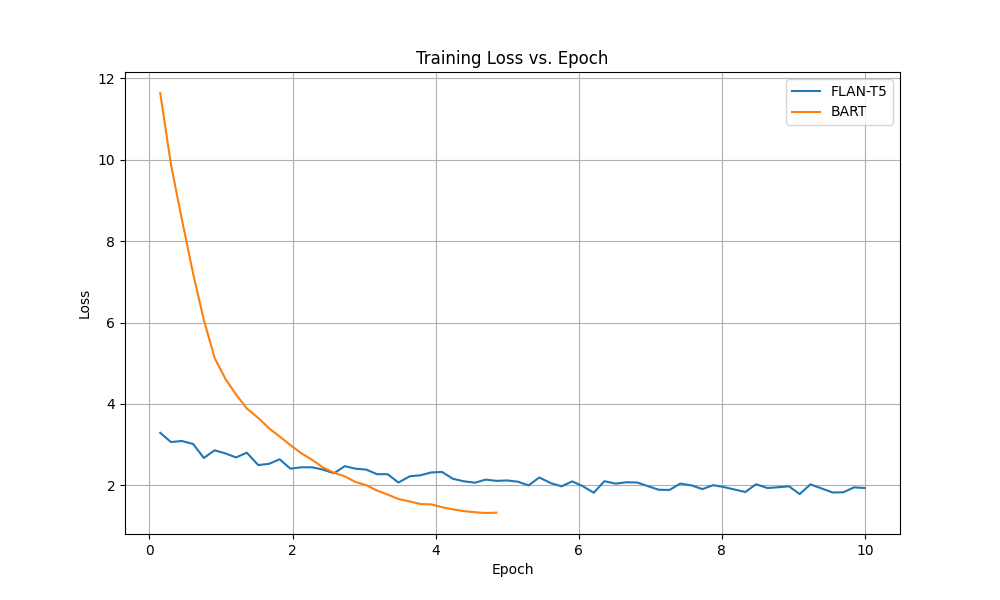
\includegraphics[width=\linewidth]{assets/train_loss.png}
    \caption{Training Loss vs Epoch}
    \label{fig:train_loss}
\end{figure}

While BART demonstrates superior performance in evaluation loss, its higher initial losses and aggressive learning suggest that it may require more extensive parameter tuning to stabilize its training process.
FLAN-T5, although slightly underperforming in evaluation, maintains a steady and predictable learning process. This could make it a more reliable choice for scenarios where stability during training is critical.

Table \ref{tab:eval_metric} compares the performance of the FLAN-T5 and BART models across three evaluation metrics.
BART achieves a higher F1 Score than FLAN-T5, suggesting BART outperforms FLAN-T5 in terms of accuracy and robustness when evaluated on token-level precision and recall.
BART also achieves a higher BLEU score than FLAN-T5, indicating that BART generates responses that are more aligned with reference outputs.
Although, FLAN-T5 is significantly faster, with an average response time of 0.976 seconds, while BART has a slower response time of 1.442 seconds.
While BART excels in performance metrics, its slower response time might limit its applicability in time-sensitive contexts.
FLAN-T5, with its efficient runtime, could be preferable for interactive or resource-constrained environments, even if it sacrifices some level of output quality.

\begin{table}[!ht]
    \centering
    \caption{Evaluation Metrics for Models}
    \label{tab:eval_metric}
    \begin{tabular}{l|c|c}
        \toprule
        \textbf{Evaluation Metric}         & \textbf{FLAN-T5}         & \textbf{BART} \\
        \midrule
        F1 Score (\%)                      & 36.094                   & 40.546                     \\ 
        BLEU Score (\%)                    & 74.275                   & 80.402                      \\ 
        Avg. Response Time (s)             & 0.976                    & 1.442                      \\
        \bottomrule
    \end{tabular}
\end{table}

%== Conclusion ==%
\section{Conclusion}
This project demonstrates the potential of leveraging small language models (SLMs) to enhance human-robot interactions in educational settings. 
By integrating FLAN-T5 or BART with microcontroller-based robotic platforms, we developed a conversational system capable of addressing prospective students' questions about department offerings, research opportunities, and more. 
Our findings indicate a trade-off between conversational accuracy and response time, with FLAN-T5 offering efficiency suited for real-time interactions and BART excelling in content accuracy and fluency.

\noindent
\textbf{Future Work:}
The most notable limitation to this project thus far is the size of the dataset. 
A large enough dataset of custom question-answer pairs could not be generated given the time limitations.
This is the first area to be worked out as development continues.
Once a larger dataset is developed, the model's hyperparameters can be fine tuned further to give more accurate and coherent responses.

Implementing this on an edge device is also to be implemented in the future. Two edge devices, Raspberry Pi and NVIDA Jetson Nano, are the target devices.
Once received, the models will be implemented and evaluated. This will help shape the development of the language models. 
Model output validation is another key area to be addressed in the future. Putting the models, current and new, though various prompt testing will highlight any areas of concern to be fixed before full implementation into a robotic system.

\begin{thebibliography}{00}
\bibitem{b1} H. Touvron et al., “Llama 2: Open foundation and fine-tuned chat models,” Jul. 2023, arXiv:2307.09288
\bibitem{b2} A. Q. Jiang et al., “Mixtral of experts,” Jan. 2024, arXiv:2401.04088.
\bibitem{b3} M. Scherer et al., "Deeploy: Enabling Energy-Efficient Deployment of Small Language Models on Heterogeneous Microcontrollers," in IEEE Transactions on Computer-Aided Design of Integrated Circuits and Systems, vol. 43, no. 11, pp. 4009-4020, Nov. 2024, doi: 10.1109/TCAD.2024.3443718.
\bibitem{b4} Mangdang, "Mangdang Store," Available: https://mangdang.store
\bibitem{b5} Poppy Project, "Poppy Humanoid," Available: https://www.poppy-project.org/en/robots/poppy-humanoid/.
\bibitem{b6} Chung, Hyung Won, Le Hou, Shayne Longpre, Barret Zoph, Yi Tay, William Fedus, Eric Li, et al. "Scaling Instruction-Finetuned Language Models." arXiv (2022). https://doi.org/10.48550/arXiv.2210.11416.
\bibitem{b7} M. Lewis, Y. Liu, N. Goyal, M. Ghazvininejad, A. Mohamed, O. Levy, V. Stoyanov, and L. Zettlemoyer, "BART: Denoising Sequence-to-Sequence Pre-training for Natural Language Generation, Translation, and Comprehension," CoRR, vol. abs/1910.13461, 2019. [Online]. Available: http://arxiv.org/abs/1910.13461.
\bibitem{b8} R. Rajpurkar, "SQuAD: The Stanford Question Answering Dataset," SQuAD Explorer.
\bibitem{b9} H. Xu, M. Scales, A. Nguyen, R. Ritter, C. Raffel, K. Shankar, S. A. Saurous, and Q. V. Le, "Deep Evolutionary Reinforcement Learning," arXiv preprint arXiv:1910.10683, 2019. [Online]. Available: https://arxiv.org/pdf/1910.10683.
\bibitem{b10} M. Lewis, Y. Liu, N. Goyal, M. Ghazvininejad, A. Mohamed, O. Levy, V. Stoyanov, and L. Zettlemoyer, "BART: Denoising Sequence-to-Sequence Pre-training for Natural Language Generation, Translation, and Comprehension," arXiv preprint arXiv:1910.13461, 2019. [Online]. Available: https://arxiv.org/pdf/1910.13461. [Accessed: Dec. 17, 2024].
\end{thebibliography}

%-- Appendix --%
\newpage
\onecolumn
\appendix
\section{Appendix}
\subsection{Sample Output from FLAN-T5 and BART} \label{sample-output}
\begin{figure*}[h]
    \centering
    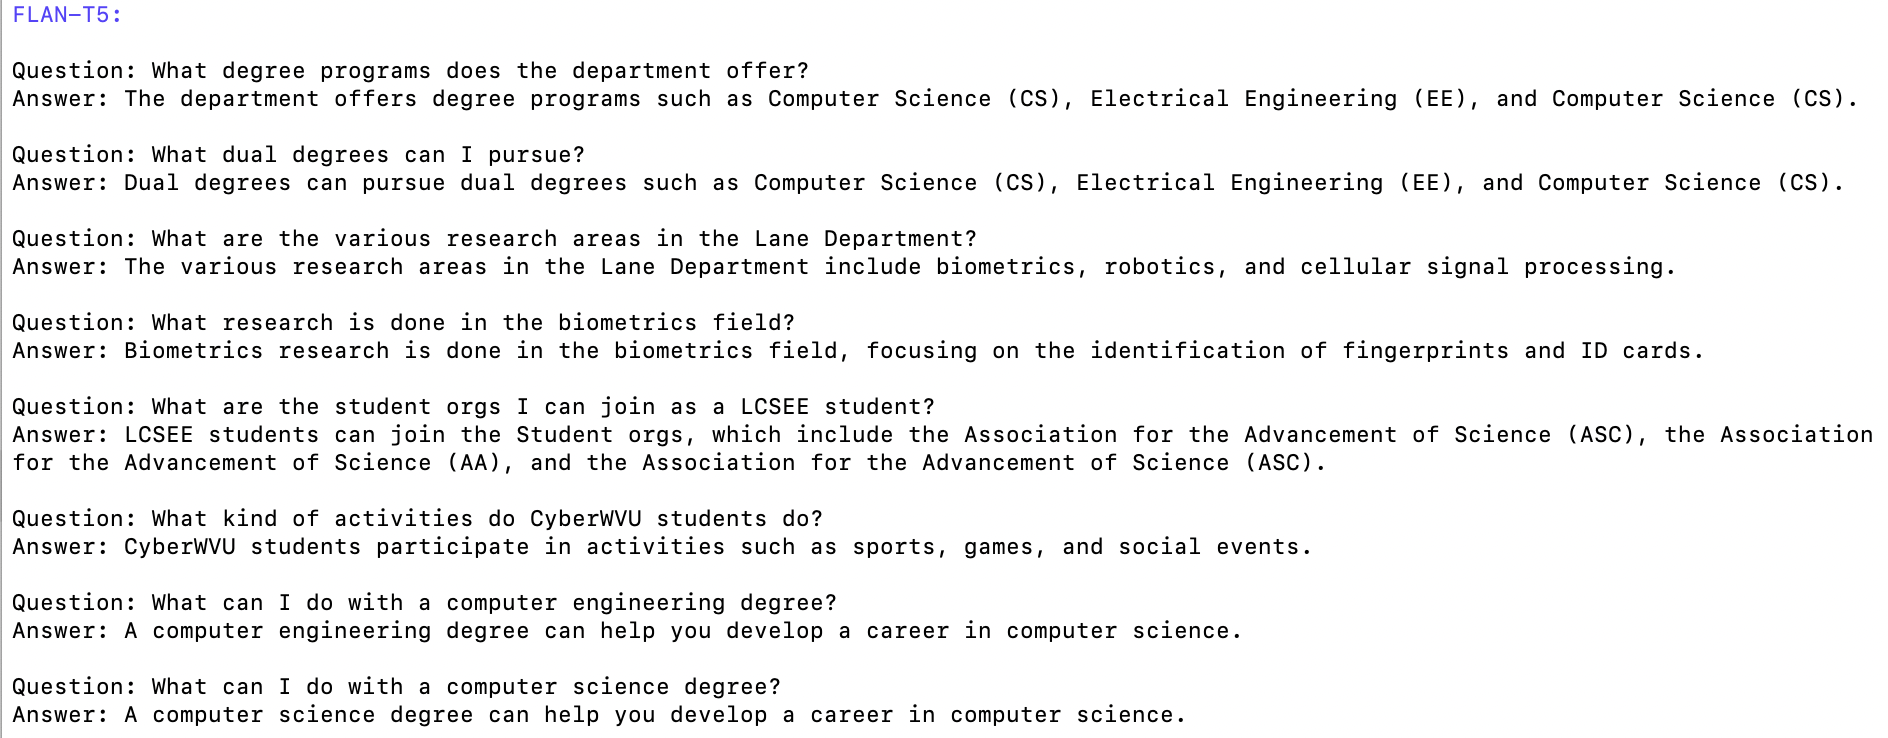
\includegraphics[width=\linewidth]{assets/Flan_out.png}
    \caption{FLAN-T5 Output}
    \label{fig:FLAN_Out}
\end{figure*}

\begin{figure*}[h]
    \centering
    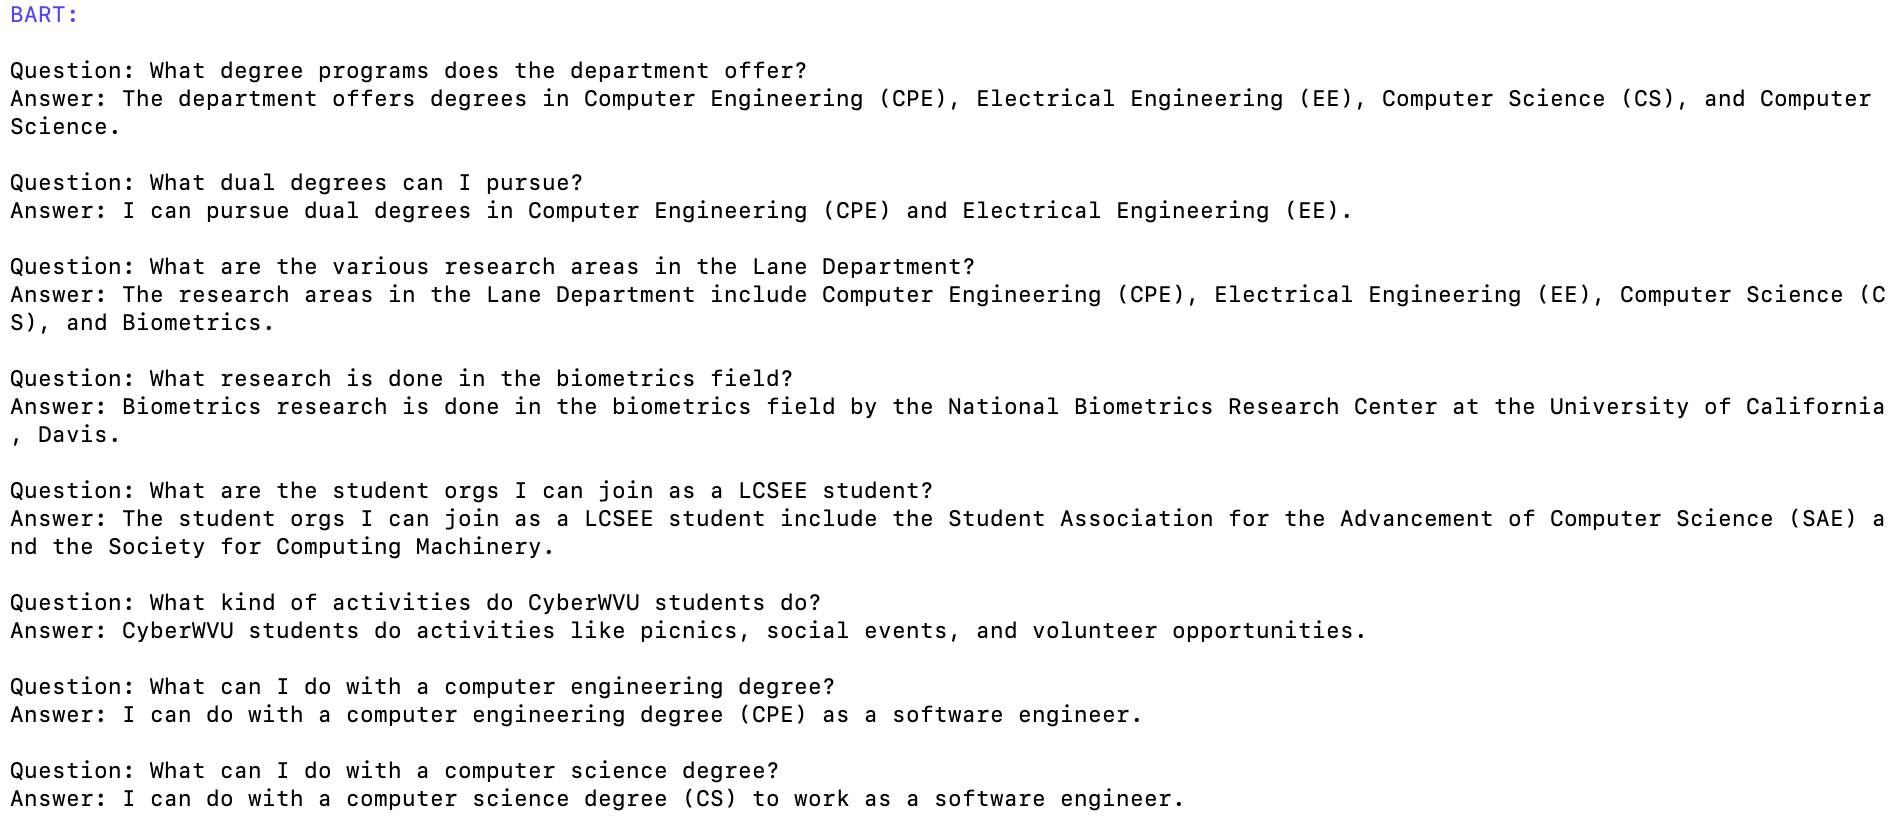
\includegraphics[width=\linewidth]{assets/Bart_out.png}
    \caption{BART Output}
    \label{fig:BART_Out}
\end{figure*}


\end{document}
